 \providecommand{\main}{../../..}
\documentclass[\main/main.tex]{subfiles}
\begin{document}
\subsection{Esercizio 1}
Dato il seguente problma di PL:

\begin{figure}
	\begin{align*}
		\max z = x_1 + x_2  \\
		x_1 + x_2  & \leq 7 \\
		x_1 - x_2  & \geq 0 \\
		x_1 + 2x_2 & \geq 2 \\
		x_1        & \leq 4 \\
		x_1, x_2   & \geq 0
	\end{align*}
	\caption{Esercizio 1}
\end{figure}

\begin{enumerate}
	\item Si disegni la regione ammissibile e si evidenzi il vertice ottimo per via grafica, riportando il valore di z e di tutte le variabili del modello.
	\item Quale caratteristica ha la soluzione così ottenuta?
	\item Si ricavi per via grafica per quali valori di $b_3$, ora pari a $2$, la \textbf{composizione} della base ottima non cambia.
	\item Si risolva mediante gli scarti complementari il duale del problema.
\end{enumerate}

\subsection{Soluzione esercizio 1}

\subsubsection*{Identifico soluzione ottima}

\begin{figure}
	\begin{subfigure}{0.49\textwidth}
		\posxyzgraph{4}{7}{x+y<= 7 && x-y>= 0 && x+y>=2}{x+y}
		\caption{Tutti i punti sul vertice tra $(3.5, 3.5)$ e $(4,3)$ sono ottimi}
	\end{subfigure}
	\begin{subfigure}{0.49\textwidth}
		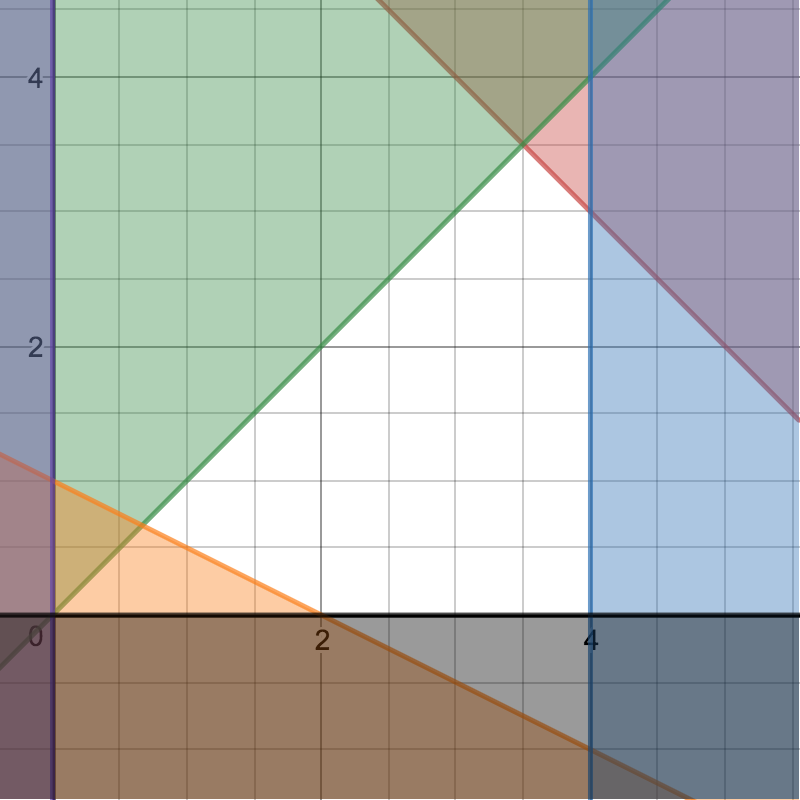
\includegraphics[width=0.9\textwidth]{2018_01_23}
		\caption{Regione di ammissibilità del problema}
	\end{subfigure}
\end{figure}

Il piano $z = x_1 + x_2$ è inclinato come il vincolo $x_1 + x_2 \leq 7$, per cui vi sono infinite soluzioni di massimo tra il vertice in $(3.5, 3.5)$ ed il vertice in $(4,3)$.

Posso scegliere quindi, \textbf{arbitrariamente}, uno dei vertici ottimi. Procedo scegliendo $\bm{x} = \begin{bmatrix}
		4 & 3
	\end{bmatrix}$.

\subsubsection*{Determino le variabili}
N.B: Le variabili di slack non possono mai essere negative.

\begin{align*}
	z   = 7,\quad
	x_1 = 4,\quad
	x_2 = 3,\quad
	s_1 = 0,\quad
	s_2 = 1,\quad
	s_3 = 8,\quad
	s_4 = 0
\end{align*}

\subsubsection*{Caratteristiche della soluzione}
La soluzione ha la caratteristiche di essere un ottimo multiplo, cioè sussistono più vertici ottimi nella regione ammissibile.

\subsubsection*{Valori di $b_2$}
Per calcolare il valore di $b_2$ è sufficiente sostituire le coordinate del vertice ottimo considerato nel vincolo.

Considerando come vertice $(4,3)$ si ottiene $b_2 = 10$ (figura \ref{2018_23_01}) mentre considerando $(3.5, 3.5)$ si ottiene $b_2 = 10.5$ (figura \ref{2018_23_02}).

Non esiste un valore inferiore di $b_2$ che va a variare la composizione della base ottima (figura \ref{2018_23_03}).

\begin{figure}
	\begin{subfigure}{0.32\textwidth}
		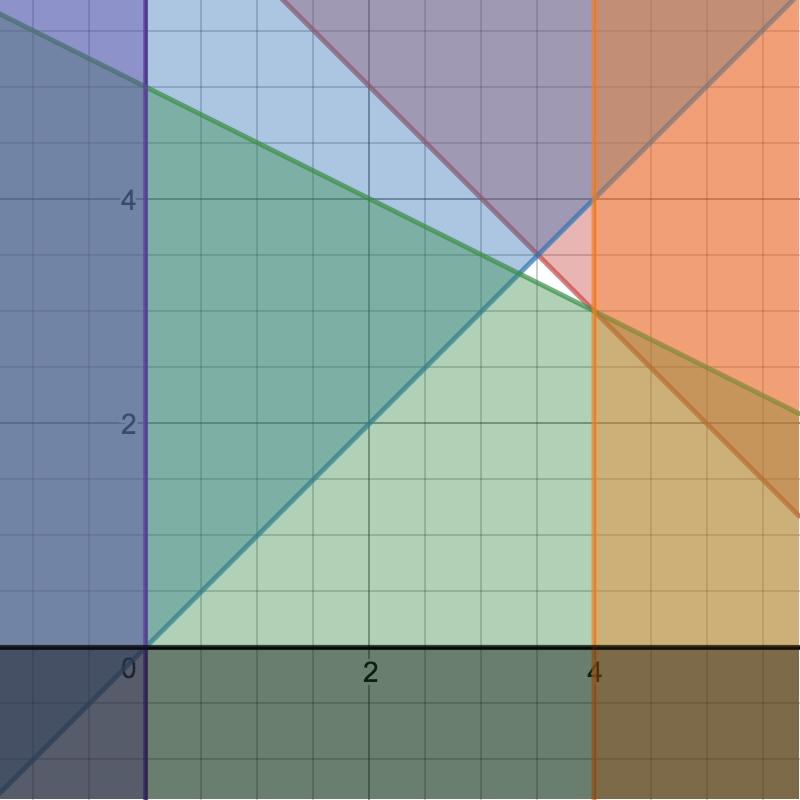
\includegraphics[width=0.9\textwidth]{2018_01_23_1}
		\caption{Caso con $b_2=10$}
		\label{2018_23_01}
	\end{subfigure}
	\begin{subfigure}{0.32\textwidth}
		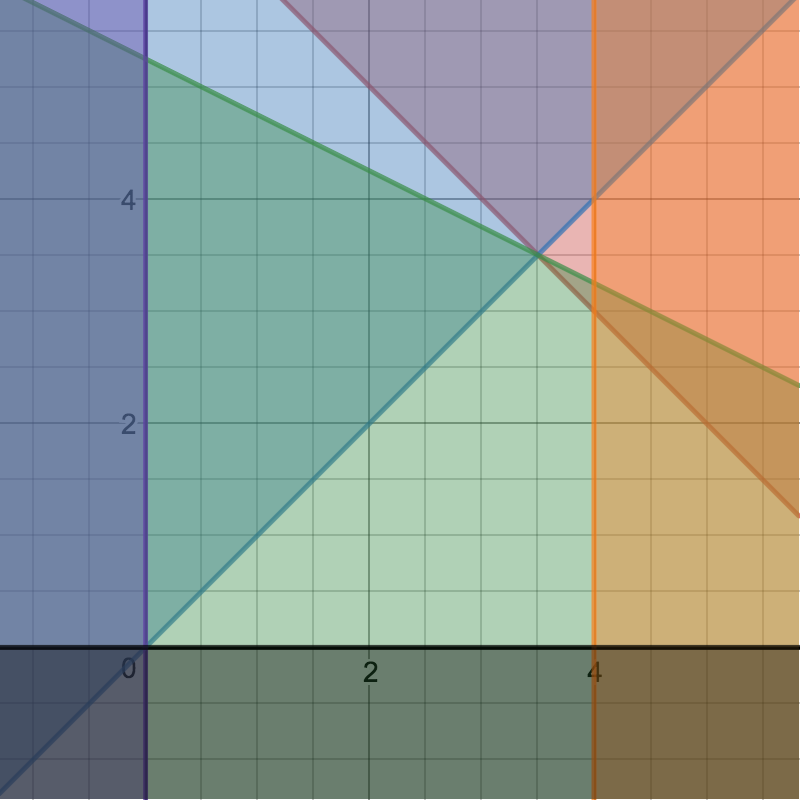
\includegraphics[width=0.9\textwidth]{2018_01_23_2}
		\caption{Caso con $b_2=10.5$}
		\label{2018_23_02}
	\end{subfigure}
	\begin{subfigure}{0.32\textwidth}
		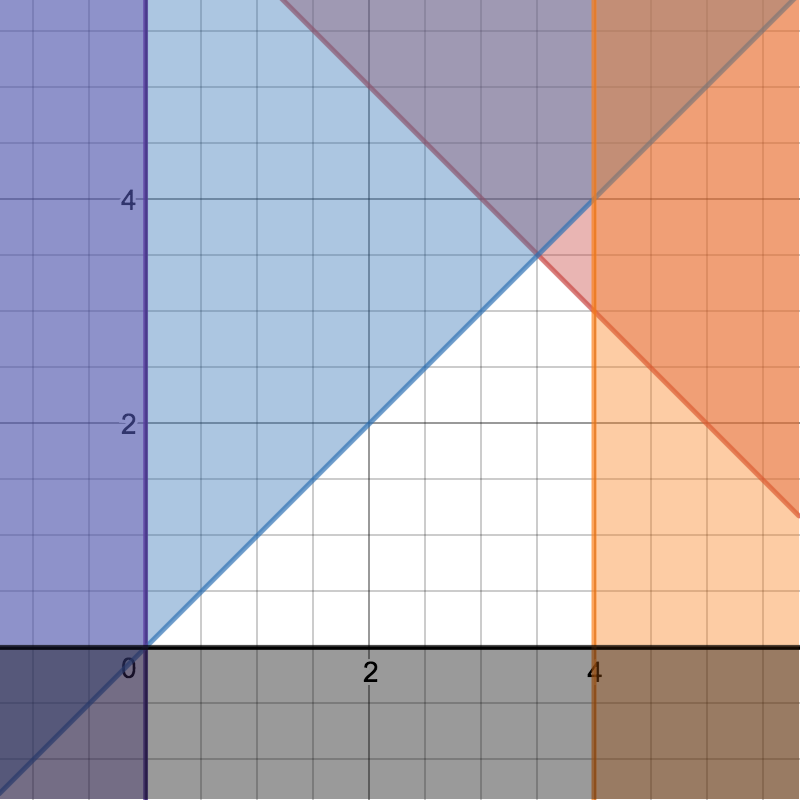
\includegraphics[width=0.9\textwidth]{2018_01_23_3}
		\caption{Caso con $b_2=-\infty$}
		\label{2018_23_03}
	\end{subfigure}
	\caption{Regione ammissibile al variare di $b_2$}
\end{figure}

\subsubsection*{Scarti complementari}
Costruisco il problema complementare:

\begin{figure}
	\begin{align*}
		\min z_D = 7y_1 + 2y_3 + 4y_4  \\
		y_1 + y_2 + y_3 + y_4 & \geq 1 \\
		y_1 - y_2 + 2y_3      & \geq 1 \\
		y_1,y_4               & \geq 0 \\
		y_2,y_3               & \leq 0 \\
	\end{align*}
	\caption{Problema complementare}
\end{figure}

Costruisco il problema degli scarti complementari:

\[
	\begin{cases}
		x_1(y_1 + y_2 + y_3 + y_4 - 1) = 0 \\
		x_2(y_1 - y_2 + 2y_3 - 1) = 0      \\
		y_1(x_1 + x_2 - 7) = 0             \\
		y_2(x_1 - x_2) = 0                 \\
		y_3(x_1 + 2x_2 -2) = 0             \\
		y_4(x_1 -4) = 0                    \\
	\end{cases}
	\Rightarrow
	\begin{cases}
		y_1 = 1 \\
		y_2 = 0 \\
		y_3 = 0 \\
		y_4 = 0 \\
	\end{cases}
\]

La soluzione ottima del problema duale è $z = z_D = 7$.

\end{document}